\documentclass[8pt]{beamer}

% Beamer style
%\usetheme[secheader]{Madrid}
% \usetheme{CambridgeUS}
\useoutertheme{infolines}
\usecolortheme[rgb={0.65,0.15,0.25}]{structure}
% \usefonttheme[onlymath]{serif}
\beamertemplatenavigationsymbolsempty
%\AtBeginSubsection

% Packages
%\usepackage[french]{babel}
\usepackage[latin1]{inputenc}
\usepackage{color}
\usepackage{xspace}
\usepackage{dsfont, stmaryrd}
\usepackage{amsmath, amsfonts, amssymb, stmaryrd}
\usepackage{epsfig}
\usepackage{tikz}
\usepackage{url}
% \usepackage{ulem}
\usepackage{/home/robin/LATEX/Biblio/astats}
%\usepackage[all]{xy}
\usepackage{graphicx}
\usepackage{xspace}

% Maths
% \newtheorem{theorem}{Theorem}
% \newtheorem{definition}{Definition}
\newtheorem{proposition}{Proposition}
% \newtheorem{assumption}{Assumption}
% \newtheorem{algorithm}{Algorithm}
% \newtheorem{lemma}{Lemma}
% \newtheorem{remark}{Remark}
% \newtheorem{exercise}{Exercise}
% \newcommand{\propname}{Prop.}
% \newcommand{\proof}{\noindent{\sl Proof:}\quad}
% \newcommand{\eproof}{$\blacksquare$}

% \setcounter{secnumdepth}{3}
% \setcounter{tocdepth}{3}
\newcommand{\pref}[1]{\ref{#1} p.\pageref{#1}}
\newcommand{\qref}[1]{\eqref{#1} p.\pageref{#1}}

% Colors : http://latexcolor.com/
\definecolor{darkred}{rgb}{0.65,0.15,0.25}
\definecolor{darkgreen}{rgb}{0,0.4,0}
\definecolor{darkred}{rgb}{0.65,0.15,0.25}
\definecolor{amethyst}{rgb}{0.6, 0.4, 0.8}
\definecolor{asparagus}{rgb}{0.53, 0.66, 0.42}
\definecolor{applegreen}{rgb}{0.55, 0.71, 0.0}
\definecolor{awesome}{rgb}{1.0, 0.13, 0.32}
\definecolor{blue-green}{rgb}{0.0, 0.87, 0.87}
\definecolor{red-ggplot}{rgb}{0.52, 0.25, 0.23}
\definecolor{green-ggplot}{rgb}{0.42, 0.58, 0.00}
\definecolor{purple-ggplot}{rgb}{0.34, 0.21, 0.44}
\definecolor{blue-ggplot}{rgb}{0.00, 0.49, 0.51}

% Commands
\newcommand{\backupbegin}{
   \newcounter{finalframe}
   \setcounter{finalframe}{\value{framenumber}}
}
\newcommand{\backupend}{
   \setcounter{framenumber}{\value{finalframe}}
}
\newcommand{\emphase}[1]{\textcolor{darkred}{#1}}
\newcommand{\comment}[1]{\textcolor{gray}{#1}}
\newcommand{\paragraph}[1]{\textcolor{darkred}{#1}}
\newcommand{\refer}[1]{{\small{\textcolor{gray}{{\cite{#1}}}}}}
\newcommand{\Refer}[1]{{\small{\textcolor{gray}{{[#1]}}}}}
\newcommand{\goto}[1]{{\small{\textcolor{blue}{[\#\ref{#1}]}}}}
\renewcommand{\newblock}{}

\newcommand{\tabequation}[1]{{\medskip \centerline{#1} \medskip}}
% \renewcommand{\binom}[2]{{\left(\begin{array}{c} #1 \\ #2 \end{array}\right)}}

% Variables 
\newcommand{\Abf}{{\bf A}}
\newcommand{\Beta}{\text{B}}
\newcommand{\Bcal}{\mathcal{B}}
\newcommand{\Bias}{\xspace\mathbb B}
\newcommand{\Cor}{{\mathbb C}\text{or}}
\newcommand{\Cov}{{\mathbb C}\text{ov}}
\newcommand{\cl}{\text{\it c}\ell}
\newcommand{\Ccal}{\mathcal{C}}
\newcommand{\cst}{\text{cst}}
\newcommand{\Dcal}{\mathcal{D}}
\newcommand{\Ecal}{\mathcal{E}}
\newcommand{\Esp}{\xspace\mathbb E}
\newcommand{\Espt}{\widetilde{\Esp}}
\newcommand{\Covt}{\widetilde{\Cov}}
\newcommand{\Ibb}{\mathbb I}
\newcommand{\Fcal}{\mathcal{F}}
\newcommand{\Gcal}{\mathcal{G}}
\newcommand{\Gam}{\mathcal{G}\text{am}}
\newcommand{\Hcal}{\mathcal{H}}
\newcommand{\Jcal}{\mathcal{J}}
\newcommand{\Lcal}{\mathcal{L}}
\newcommand{\Mt}{\widetilde{M}}
\newcommand{\mt}{\widetilde{m}}
\newcommand{\Nbb}{\mathbb{N}}
\newcommand{\Mcal}{\mathcal{M}}
\newcommand{\Ncal}{\mathcal{N}}
\newcommand{\Ocal}{\mathcal{O}}
\newcommand{\pt}{\widetilde{p}}
\newcommand{\Pt}{\widetilde{P}}
\newcommand{\Pbb}{\mathbb{P}}
\newcommand{\Pcal}{\mathcal{P}}
\newcommand{\Qcal}{\mathcal{Q}}
\newcommand{\qt}{\widetilde{q}}
\newcommand{\Rbb}{\mathbb{R}}
\newcommand{\Sbb}{\mathbb{S}}
\newcommand{\Scal}{\mathcal{S}}
\newcommand{\st}{\widetilde{s}}
\newcommand{\St}{\widetilde{S}}
\newcommand{\Tcal}{\mathcal{T}}
\newcommand{\todo}{\textcolor{red}{TO DO}}
\newcommand{\Ucal}{\mathcal{U}}
\newcommand{\Un}{\math{1}}
\newcommand{\Vcal}{\mathcal{V}}
\newcommand{\Var}{\mathbb V}
\newcommand{\Vart}{\widetilde{\Var}}
\newcommand{\Zcal}{\mathcal{Z}}

% Symboles & notations
\newcommand\independent{\protect\mathpalette{\protect\independenT}{\perp}}\def\independenT#1#2{\mathrel{\rlap{$#1#2$}\mkern2mu{#1#2}}} 
\renewcommand{\d}{\text{\xspace d}}
\newcommand{\gv}{\mid}
\newcommand{\ggv}{\, \| \, }
% \newcommand{\diag}{\text{diag}}
\newcommand{\card}[1]{\text{card}\left(#1\right)}
\newcommand{\trace}[1]{\text{tr}\left(#1\right)}
\newcommand{\matr}[1]{\boldsymbol{#1}}
\newcommand{\matrbf}[1]{\mathbf{#1}}
\newcommand{\vect}[1]{\matr{#1}} %% un peu inutile
\newcommand{\vectbf}[1]{\matrbf{#1}} %% un peu inutile
\newcommand{\trans}{\intercal}
\newcommand{\transpose}[1]{\matr{#1}^\trans}
\newcommand{\crossprod}[2]{\transpose{#1} \matr{#2}}
\newcommand{\tcrossprod}[2]{\matr{#1} \transpose{#2}}
\newcommand{\matprod}[2]{\matr{#1} \matr{#2}}
\DeclareMathOperator*{\argmin}{arg\,min}
\DeclareMathOperator*{\argmax}{arg\,max}
\DeclareMathOperator{\sign}{sign}
\DeclareMathOperator{\tr}{tr}
\newcommand{\ra}{\emphase{$\rightarrow$} \xspace}

% Hadamard, Kronecker and vec operators
\DeclareMathOperator{\Diag}{Diag} % matrix diagonal
\DeclareMathOperator{\diag}{diag} % vector diagonal
\DeclareMathOperator{\mtov}{vec} % matrix to vector
\newcommand{\kro}{\otimes} % Kronecker product
\newcommand{\had}{\odot}   % Hadamard product

% TikZ
\newcommand{\nodesize}{2em}
\newcommand{\edgeunit}{2.5*\nodesize}
\newcommand{\edgewidth}{1pt}
\tikzstyle{node}=[draw, circle, fill=black, minimum width=.75\nodesize, inner sep=0]
\tikzstyle{square}=[rectangle, draw]
\tikzstyle{param}=[draw, rectangle, fill=gray!50, minimum width=\nodesize, minimum height=\nodesize, inner sep=0]
\tikzstyle{hidden}=[draw, circle, fill=gray!50, minimum width=\nodesize, inner sep=0]
\tikzstyle{hiddenred}=[draw, circle, color=red, fill=gray!50, minimum width=\nodesize, inner sep=0]
\tikzstyle{observed}=[draw, circle, minimum width=\nodesize, inner sep=0]
\tikzstyle{observedred}=[draw, circle, minimum width=\nodesize, color=red, inner sep=0]
\tikzstyle{eliminated}=[draw, circle, minimum width=\nodesize, color=gray!50, inner sep=0]
\tikzstyle{empty}=[draw, circle, minimum width=\nodesize, color=white, inner sep=0]
\tikzstyle{blank}=[color=white]
\tikzstyle{nocircle}=[minimum width=\nodesize, inner sep=0]

\tikzstyle{edge}=[-, line width=\edgewidth]
\tikzstyle{edgebendleft}=[-, >=latex, line width=\edgewidth, bend left]
\tikzstyle{edgebendright}=[-, >=latex, line width=\edgewidth, bend right]
\tikzstyle{lightedge}=[-, line width=\edgewidth, color=gray!50]
\tikzstyle{lightedgebendleft}=[-, >=latex, line width=\edgewidth, bend left, color=gray!50]
\tikzstyle{lightedgebendright}=[-, >=latex, line width=\edgewidth, bend right, color=gray!50]
\tikzstyle{edgered}=[-, line width=\edgewidth, color=red]
\tikzstyle{edgebendleftred}=[-, >=latex, line width=\edgewidth, bend left, color=red]
\tikzstyle{edgebendrightred}=[-, >=latex, line width=\edgewidth, bend right, color=red]

\tikzstyle{arrow}=[->, >=latex, line width=\edgewidth]
\tikzstyle{arrowbendleft}=[->, >=latex, line width=\edgewidth, bend left]
\tikzstyle{arrowbendright}=[->, >=latex, line width=\edgewidth, bend right]
\tikzstyle{arrowred}=[->, >=latex, line width=\edgewidth, color=red]
\tikzstyle{arrowbendleftred}=[->, >=latex, line width=\edgewidth, bend left, color=red]
\tikzstyle{arrowbendrightred}=[->, >=latex, line width=\edgewidth, bend right, color=red]
\tikzstyle{arrowblue}=[->, >=latex, line width=\edgewidth, color=blue]
\tikzstyle{dashedarrow}=[->, >=latex, dashed, line width=\edgewidth]
\tikzstyle{dashededge}=[-, >=latex, dashed, line width=\edgewidth]
\tikzstyle{dashededgebendleft}=[-, >=latex, dashed, line width=\edgewidth, bend left]
\tikzstyle{lightarrow}=[->, >=latex, line width=\edgewidth, color=gray!50]

\newcommand{\GMSBM}{/home/robin/RECHERCHE/RESEAUX/EXPOSES/1903-SemStat/}
\newcommand{\figeconet}{/home/robin/RECHERCHE/ECOLOGIE/EXPOSES/1904-EcoNet-Lyon/Figs}
\newcommand{\fignet}{/home/robin/RECHERCHE/RESEAUX/EXPOSES/FIGURES}
\newcommand{\figeco}{/home/robin/RECHERCHE/ECOLOGIE/EXPOSES/FIGURES}
\newcommand{\figbayes}{/home/robin/RECHERCHE/BAYES/EXPOSES/FIGURES}
\newcommand{\figCMR}{/home/robin/Bureau/RECHERCHE/ECOLOGIE/CountPCA/sparsepca/Article/Network_JCGS/trunk/figs}
\newcommand{\figtree}{/home/robin/RECHERCHE/BAYES/VBEM-IS/VBEM-IS.git/Data/Tree/Fig}

\renewcommand{\nodesize}{1.75em}
\renewcommand{\edgeunit}{2.25*\nodesize}

%====================================================================
%====================================================================
\begin{document}
%====================================================================
%====================================================================

\title{Models with latent variables for community ecology}

\author[S. Robin]{S. Robin \\ ~\\
  {\small INRAE / AgroParisTech / univ. Paris-Saclay / MNHN} \\ ~\\
  joint work with J. Chiquet, S. Donnet, M. Mariadassou, \dots}

\date{Oct'20, Bordeaux}

\maketitle

%====================================================================
\frame{\frametitle{Community ecology}

{\sl Community ecology [\dots] is the study of the interactions between species in communities [\dots].} \Refer{Wikipedia}

\pause \bigskip \bigskip
\paragraph{Need for statistical models to}
\begin{itemize}
 \item \bigskip decipher / describe / evaluate environmental effects on species ({\sl abiotic} interactions) and between species interactions ({\sl biotic} interactions) \\ ~\\
 \ra \emphase{joint species distribution models}
 \item \bigskip describe / understand the organisation of species interaction networks \\ ~\\
  \ra \emphase{network models}
\end{itemize}

}

%====================================================================
\frame{\frametitle{Outline} \tableofcontents}

%====================================================================
%====================================================================
\section{Two models with latent variables}
\frame{\frametitle{Outline} \tableofcontents[currentsection]}
%====================================================================
\subsection[Joint species distribution models]{Joint species distribution models: Poisson log-normal}
%====================================================================
\frame{\frametitle{Joint species distribution models (JDSM)} \pause

  \begin{tabular}{cc}
    \hspace{-.04\textwidth}
    \begin{tabular}{p{.5\textwidth}}
      \paragraph{Fish species in Barents sea \refer{FNA06}:} 
      \begin{itemize}
       \item $89$ sites (stations), 
       \item $30$ fish species, 
       \item $4$ covariates 
      \end{itemize}

      \bigskip \bigskip 
      \paragraph{Questions:} 

      \begin{itemize}
       \item Do environmental conditions affect species abundances? (abiotic) \\~ 
       \item Do species abundances vary independently? (biotic)
      \end{itemize} 
      
      \bigskip
      See \refer{WBO15}
    \end{tabular}
    &
    \begin{tabular}{p{.45\textwidth}}
      \paragraph{Abundance table:} ~ \\
        {\footnotesize \begin{tabular}{rrrr}
        {\sl Hi.pl} & {\sl An.lu} & {\sl Me.ae} & \dots \\
%         \footnote{{\sl Hi.pl}: Long rough dab, {\sl An.lu}: Atlantic wolffish, {\sl Me.ae}: Haddock} \\ 
  %       Dab & Wolffish & Haddock \\ 
        \hline
        31  &   0  & 108 & \\
         4  &   0  & 110 & \\
        27  &   0  & 788 & \\
        13  &   0  & 295 & \\
        23  &   0  &  13 & \\
        20  &   0  &  97 & \\
        . & . & . & 
      \end{tabular}} 
      \\
      \bigskip \bigskip 
      \paragraph{Environmental covariates:} ~ \\
        {\footnotesize \begin{tabular}{rrrr}
        Lat. & Long. & Depth & Temp. \\
        \hline
        71.10 & 22.43 & 349 & 3.95 \\
        71.32 & 23.68 & 382 & 3.75 \\
        71.60 & 24.90 & 294 & 3.45 \\
        71.27 & 25.88 & 304 & 3.65 \\
        71.52 & 28.12 & 384 & 3.35 \\
        71.48 & 29.10 & 344 & 3.65 \\
        . & . & . & .
      \end{tabular}} 
    \end{tabular}
  \end{tabular}
  
}

%====================================================================
\frame{\frametitle{Poisson log-normal model (PLN)}
 
  \begin{tabular}{cc}
    \hspace{-.04\textwidth}
    \begin{tabular}{p{.5\textwidth}}
      \paragraph{Data:} 
      \begin{itemize}
       \item $n$ sites, $p$ species, $d$ covariates 
       \item Abundance table: ${Y} = [Y_{ij}]$
       \item Covariate table: ${X} = [x_{ik}]$
      \end{itemize}
 
      \bigskip \bigskip \bigskip 
      \paragraph{PLN model:} \refer{AiH89}
      \begin{itemize}
       \item \emphase{$Z_i =$ latent vector} associated with site $i$
       $$
       Z_i \sim \Ncal_p(0, {\Sigma})
       $$
       \item $Y_{ij} = $ observed abundance for species $j$ in site $i$
       $$
       Y_{ij} \sim \Pcal(\exp(x_i^\intercal {\beta_j} + Z_{ij}))
       $$
      \item ${\theta} = (\beta, \Sigma)$
      \end{itemize}
    \end{tabular}
    & \pause
    \begin{tabular}{p{.45\textwidth}}
      \paragraph{Covariance matrix $\widehat{\Sigma}$:} biotic \\ 
      \includegraphics[width=.3\textwidth]{\figeco/BarentsFish-corrAll} \\
      ~\\
      \paragraph{Regression cofficients $\widehat{\beta}$:} abiotic \\ 
      \includegraphics[width=.3\textwidth]{\figeco/BarentsFish-coeffAll}
    \end{tabular}    
  \end{tabular}
 
}

%====================================================================
\subsection[Models for species interaction networks]{Models for species interaction networks: Stochastic block model}
%====================================================================
\frame{\frametitle{Models for species interaction networks} \pause

  \begin{tabular}{cc}
    \hspace{-.04\textwidth}
    \begin{tabular}{p{.5\textwidth}}
      \paragraph{Tree species interactions \refer{VPD08}:} 
      \begin{itemize}
       \item $n = 51$ tree species
       \item $Y_{ij} =$ number of fungal parasites shared by species $i$ and $j$
       \item $x_{ij} =$ vector of similarities (taxonomic, geographic, genetic) between species $i$ and $j$
      \end{itemize}
      
      \bigskip \bigskip
      \paragraph{Questions:} 
      \begin{itemize}
       \item Is the network 'organized' in some way? \\~
       \item Do the covariate contribute to explain why species interact?
      \end{itemize}

      
%       \bigskip \bigskip 
%       \paragraph{Other types of network.} 
%       \begin{itemize}
%       \item plant-pollinator: mutualistic network (bipartite) 
%       \item predator-prey: trophic network (multipartite)
%       \end{itemize}
    \end{tabular}
    &
    \begin{tabular}{p{.45\textwidth}}
      \paragraph{Network (weighted):} \\
%       \includegraphics[height=.25\textwidth,width=.25\textwidth,trim=30 30 30 30]     
      \includegraphics[height=.3\textwidth,width=.3\textwidth]{\fignet/Tree-netCircle}
 \\
      \paragraph{Adjacency matrix (counts):} \\
      \includegraphics[height=.3\textwidth,width=.3\textwidth]{\fignet/Tree-adjMat}
    \end{tabular}
  \end{tabular}
      
}

%====================================================================
\frame{\frametitle{Stochastic block models (SBM)}

  \begin{tabular}{cc}
    \hspace{-.04\textwidth}
    \begin{tabular}{p{.5\textwidth}}
      \paragraph{Data:} 
      \begin{itemize}
       \item $n$ species, $d$ covariates
       \item Adjacency matrix: ${Y} = [Y_{ij}]$
       \item Covariate matrices: ${X^1, \dots X^d}$
      \end{itemize}
      \bigskip \bigskip 
      \paragraph{Stochastic block model:} \refer{HoL79} $K$ groups, 

      \begin{itemize}
      \item \emphase{$Z_i =$ latent variable} indicating to which group node $i$ belongs to
      $$
      \Pr\{Z_i = k\} = {\pi_k}
      $$
      \item $Y_{ij} =$ observed number of interactions between species $i$ and $j$
      $$
      Y_{ij} \mid Z_i, Z_j \sim \Pcal(\exp(x_{ij}^\intercal {\beta} + \alpha_{Z_i Z_j}))
      $$
      \item ${\theta} = (\pi, \alpha, \beta)$ \qquad (and $K$)
      \end{itemize}
    \end{tabular}
    &
    \begin{tabular}{p{.45\textwidth}}
      \paragraph{Observed adjacency matrix:} \\
      \includegraphics[height=.3\textwidth,width=.3\textwidth]{\fignet/Tree-adjMat} \\
      \pause
      \paragraph{Clustered matrix:} (no covariate) \\
      \includegraphics[height=.3\textwidth,width=.3\textwidth]{\fignet/Tree-adjMat-SBMnull}
    \end{tabular}
  \end{tabular}

}

%====================================================================
%====================================================================
\section{(Variational) inference of incomplete data models}
\frame{\frametitle{Outline} \tableofcontents[currentsection]}
%====================================================================
\subsection*{A reminder on the EM algorithm}
%====================================================================
\frame{\frametitle{A reminder on the EM algorithm} 

  \paragraph{Maximum likelihood inference.}
  $$
  \widehat{\theta} = \arg\max_\theta \; \log p(Y; \theta)
  $$
  \ra no closed form for ${p(Y; \theta) = \int \underset{\text{complete likelihood}}{\underbrace{p(Y, Z; \theta)}} \d Z}$ in latent variable models

  \pause \bigskip \bigskip
  \paragraph{Incomplete data models.} EM algorithm \refer{DLR77}
  $$
  \log p(Y; \theta) 
  = \underset{\text{\normalsize \emphase{M step}}}{\underbrace{\Esp(\log p(Y, Z; \theta) \mid Y)}} 
  - \Esp(\log \underset{\text{\normalsize \emphase{E step}}}{\underbrace{p(Z \mid Y; \theta)}} \mid Y)
  $$
  
%   \pause \bigskip
%   \paragraph{Expectation-maximisation algorithm.}
%   \begin{description}
%    \item[E step:] Evaluate (some moments of) $p(Z \mid Y)$
%    \item[M step:] Maximize $\Esp(\log p(Y, Z; \theta) \mid Y )$ with respect to $\theta$
%   \end{description}

  \pause \bigskip \bigskip
  \paragraph{Critical step: E step.} Evaluate $p(Z \mid Y; \theta)$
  \begin{itemize}
  \item easy: mixture models, Gaussian mixed-models
  \item use a trick: hidden Markov models, phylogenetic models
  \item intractable: many models, including PLN \& SBM
  \end{itemize}
}

%====================================================================
\subsection*{Variational EM algorithms}
%====================================================================
\frame{\frametitle{Variational approximation} 

  \paragraph{Twisted problem:} \refer{Jaa01,WaJ08,BKM17} maximize the lower bound
  \begin{align*}
  J(\theta, q)
  & = \log p(Y; \theta) 
  - \underset{\text{\normalsize {VE step}}}{\underbrace{\emphase{KL(q(Z) \mid\mid p(Z \mid Y))}}} \\
  & = 
  \underset{\text{\normalsize {M step}}}{\underbrace{\emphase{\Esp_q (\log p(Y, Z; \theta))}}} 
  - \Esp_q(\log q(Z)) 
  \end{align*}
  where $q(Z) \simeq p(Z \mid Y)$ is chosen within a \emphase{class of distributions $\Qcal$}
  
  \pause \bigskip \bigskip
  \paragraph{Many avatars.} 
  \begin{itemize}
    \item Alternative divergences: $\alpha$-divergences \refer{Min05}, $KL(p(Z \mid Y) \mid\mid q(Z))$\footnote{$KL(p \mid\mid q) = \Esp_p \log(p/q)$} (expectation-propagation = EP \refer{Min01}) 
    \item Bayesian inference (variational Bayes = VB): look for $q(\theta) \simeq p(\theta \mid Y)$ 
    \item Bayesian inference for incomplete data model (VBEM): $q(\theta, Z) \simeq p(\theta, Z \mid Y)$ \refer{BeG03} 
  \end{itemize} 
  
  \bigskip
  \ra Reasonably easy to implement and computationally efficient
  
}

%====================================================================
\frame{\frametitle{Approximate distribution} 

  \paragraph{Critical choice:} $\Qcal$ needs to be \\ ~
  \begin{itemize}
  \item 'large' enough to include good approximations of $p(Z \mid Y)$ \\ ~
  \item 'small' enough to make the calculations tractable
  \end{itemize}
  
  \pause \bigskip \bigskip
  \paragraph{Examples:} 
  \begin{itemize}
   \item PLN model for species abundance: $$\Qcal := \{\text{multivariate Gaussian distributions}\}$$ \\~
   \item SBM model for networks: $$\Qcal := \{\text{factorable discrete distributions}\}$$ \\
   ('mean-field' approximation)
  \end{itemize}

}

%====================================================================
%====================================================================
\section{Various use of joint species distribution models}
\frame{\frametitle{Outline} \tableofcontents[currentsection]}
%====================================================================
\subsection*{Poisson log-normal model}
%====================================================================
\frame{\frametitle{Poisson log-normal model} 

  \begin{tabular}{cc}
    \hspace{-.04\textwidth}
    \begin{tabular}{p{.45\textwidth}}
      \paragraph{Barents' fish:} $n = 89$ sites, $p = 30$ species \\
      
      \bigskip 
      \paragraph{$Y =$ abundances:} ~ \\
        {\footnotesize \begin{tabular}{rrrr}
        {\sl Hi.pl} & {\sl An.lu} & {\sl Me.ae} & \dots \\
%         \footnote{{\sl Hi.pl}: Long rough dab, {\sl An.lu}: Atlantic wolffish, {\sl Me.ae}: Haddock} \\ 
  %       Dab & Wolffish & Haddock \\ 
        \hline
        31  &   0  & 108 & \\
         4  &   0  & 110 & \\
        27  &   0  & 788 & \\
        13  &   0  & 295 & \\
        23  &   0  &  13 & \\
        20  &   0  &  97 & \\
        . & . & . & 
      \end{tabular}} 
      \\
      \bigskip
      \paragraph{$X =$ covariates:} ~ \\
        {\footnotesize \begin{tabular}{rrrr}
        Lat. & Long. & Depth & Temp. \\
        \hline
        71.10 & 22.43 & 349 & 3.95 \\
        71.32 & 23.68 & 382 & 3.75 \\
        71.60 & 24.90 & 294 & 3.45 \\
        71.27 & 25.88 & 304 & 3.65 \\
        71.52 & 28.12 & 384 & 3.35 \\
        71.48 & 29.10 & 344 & 3.65 \\
        . & . & . & .
      \end{tabular}} 
      \bigskip ~
      \bigskip ~
    \end{tabular}
    &
    \begin{tabular}{p{.5\textwidth}}
      \pause
      \paragraph{Join species distribution model.}
      \begin{itemize}
       \item $n$ independent sites
       \item $Z_i=$ latent vector for site $i$
       $$
       Z_i \sim \Ncal(0, \Sigma)
       $$
       \item $x_i =$ vector of covariates for site $i$
       \item $Y_{ij} =$ abundance of species $j$ in site $i$:
       $$
       Y_{ij} \sim \Pcal(\exp(x_i^\intercal \beta_j + Z_{ij}))
       $$
      \end{itemize}
      
      \pause \bigskip
      \paragraph{Interpretation:}
      \begin{itemize}
       \item $\Sigma:$ biotic interactions 
       \item $\beta:$ abiotic effects 
      \end{itemize}
 
      \bigskip \bigskip
      \paragraph{Desirable properties:}
      \begin{itemize}
      \item $\Var(Y_{ij}) > \Var(\Pcal(\exp(x_i^\intercal \beta_j))$
      \item $\sign(\sigma_{jk}) = \sign(\Cor(Y_{ij}, Y_{ik}))$ 
      \end{itemize}
    \end{tabular}
  \end{tabular}
  
}

%====================================================================
\frame{\frametitle{VEM inference} 

  \paragraph{Variational approximation.} $\Qcal = \{\text{multivariate Gaussian}\}$
  $$
  p(Z_i \mid Y_i) \simeq q_i(Z_i) := \Ncal(Z_i; {m_i, S_i}), 
  $$
  $(m_i, S_i)_{1 \leq i \leq n}$ = {\sl variational parameters}.
  
  \pause \bigskip \bigskip
  \paragraph{VE step:} minimize wrt $(m_i, S_i)_{1 \leq i \leq n}$
  $$
  KL(q(Z) \mid\mid p(Z \mid Y; \theta)) = KL(q(Z) \mid\mid p(Z, Y; \theta)) + \text{cst}
  $$
  \ra convex problem
  
  \pause \bigskip \bigskip
  \paragraph{M step:} maximize wrt $\theta = (\beta, \Sigma)$
  $$
  \Esp_q (\log p(Y, Z; \theta))
  $$
  \ra convex problem (weighted GLM)
}

%====================================================================
\frame{\frametitle{Abiotic vs biotic interactions} 

%   \paragraph{Variational EM \refer{CMR18a,CMR19}:} $p(Z_i \mid Y_i) \simeq \Ncal(Z_i; m_i, S_i)$
  
%   \pause \bigskip 
  \begin{tabular}{cc|c}
    \multicolumn{2}{l|}{\emphase{Full model}} &
    \multicolumn{1}{l}{\emphase{Null model}} \\
    & & \\
    \multicolumn{2}{c|}{{$Y_{ij} \sim \Pcal(\exp(\emphase{x_i^\intercal \beta_j} + Z_{ij}))$}} &
    \multicolumn{1}{c}{{$Y_{ij} \sim \Pcal(\exp(\emphase{\mu_j} + Z_{ij}))$}} \\
    & & \\
    \multicolumn{2}{l|}{{$x_i =$ all covariates}} &
    \multicolumn{1}{l}{{no covariate}} \\ 
    & & \\
    & correlations between & \\
    inferred  correlations $\widehat{\Sigma}_{\text{full}}$ & 
    predictions: $x_i^\intercal \widehat{\beta}_j$ & 
    inferred correlations $\widehat{\Sigma}_{\text{null}}$ \\ 
    \includegraphics[width=.3\textwidth, trim=20 20 20 20]{\figeco/BarentsFish-corrAll} 
    &
    \includegraphics[width=.3\textwidth, trim=20 20 20 20]{\figeco/BarentsFish-corrPred} &
    \includegraphics[width=.3\textwidth, trim=20 20 20 20]{\figeco/BarentsFish-corrNull}
  \end{tabular}

}

%====================================================================
\frame{\frametitle{Ease of modeling with latent variables} 

  \paragraph{Latent layer = multivariate Gaussian:} flexible dependency structure (\url{PLNmodels} package) \refer{CMR20}
  
  \pause \bigskip \bigskip
  \paragraph{Dimension reduction.} 
  \begin{itemize}
  \item Metagenomic, metabarcoding, environmental genomics: $p = 10^2, 10^3$ species
  \item Probabilistic PCA \refer{Tib99}: suppose that \emphase{$\Sigma$ has rank $r \ll p$}
  \item PLN-PCA: PLN model with rank constraint on $\Sigma$ \refer{CMR18a}
  \end{itemize}
  
  \pause \bigskip \bigskip
  \paragraph{Network inference.} 
  \begin{itemize}
  \item $\Sigma$ include both direct and indirect interactions
  \item Gaussian graphical models: \emphase{$\Sigma^{-1}$ should be sparse}
  \item PLN-network: PLN model with graphical lasso penalty \refer{CMR19}
  \end{itemize}
  $$
  \arg\max_{\beta, \Sigma, q \in \Qcal} \; 
  \underset{{\text{\normalsize log-likelihood}}}{\underbrace{\log p(Y; \beta, \Sigma)}}
  - \underset{{\text{\normalsize variational approx.}}}{\underbrace{KL(q(Z) \mid\mid p(Z \mid Y))}}
  - \underset{{\text{\normalsize $\ell_1$ penalty}}}{\underbrace{\emphase{\lambda \|\Sigma^{-1}\|_1}}}
  $$
  
}

%====================================================================
\frame{\frametitle{PLN for dimension reduction (PCA)}

  \begin{tabular}{cl}
    \hspace{-.04\textwidth}
    \begin{tabular}{p{.3\textwidth}}
      \paragraph{Metabarcoding data} \refer{JFS16} \\ ~
      \begin{itemize}
      \item $p = 114$ OTUs (bacteria and fungi) \\ ~
      \item $n = 116$ leaves \\ ~
      \item collected on 3 trees 
        \begin{itemize}
        \item resistant 
        \item intermediate
        \item susceptible       
      \end{itemize}
      to oak powdery mildew
      \end{itemize}

      \bigskip \bigskip 
      \paragraph{Model selection:} 
      \begin{itemize}
        \item Penalized lower-bound $J(\widehat{\theta}, \widehat{q})$ \\
        (pseudo BIC, pseudo ICL, \dots)
      \end{itemize}

    \end{tabular}
    &
    \begin{tabular}{p{.55\textwidth}}
    \includegraphics[height=.4\textheight]{\fignet/CMR18-AnnApplStat-Fig4a} \\
    ~ \\
    \includegraphics[height=.4\textheight]{\fignet/CMR18-AnnApplStat-Fig5a} 
    \end{tabular}
  \end{tabular}
}

%====================================================================
\frame{\frametitle{Network inference (Barents' fish species)} 
  
  \vspace{-.05\textheight}
  $$
  \includegraphics[height=.85\textheight]{\fignet/CMR18b-ArXiv-Fig5}
  $$
  }

%====================================================================
\frame{\frametitle{PLN for network inference: choosing $\lambda$}

  $$
  \includegraphics[height=.8\textheight]{\fignet/BarentsFish_Gfull_criteria}
  $$
}

%====================================================================
%====================================================================
\section{Inference of network models}
\frame{\frametitle{Outline} \tableofcontents[currentsection]}
%====================================================================
\subsection*{Stochastic blockmodel}
%====================================================================
\frame{\frametitle{Stochastic block models (SBM)}

%   \vspace{-0.05\textheight}
  \begin{tabular}{cc}
    \hspace{-.04\textwidth}
    \begin{tabular}{c}
      \paragraph{Observed network:} (adjacency matrix) \\
      \includegraphics[height=.25\textwidth,width=.25\textwidth, trim=20 20 20 20]{\fignet/Tree-adjMat} \\ ~ \\
      \paragraph{Clustered matrix (no covariate):} \\
      \includegraphics[height=.25\textwidth,width=.25\textwidth, trim=20 20 20 20]{\fignet/Tree-adjMat-SBMnull}
    \end{tabular}
    &
    \begin{tabular}{p{.5\textwidth}}
      \pause
      \paragraph{Network model.}
      \begin{itemize}
        \item $n$ species, $d$ covariates, $K$ groups
        \item $Z_i=$ latent group of species $i$
        $$
        \Pr\{Z_i = k\} = \pi_k
        $$
        \item $x_{ij} =$ vector of covariates for species $(i, j)$
        \item $Y_{ij} =$ observed nb of interactions $(i, j)$ % $i$ and $j$
        $$
        Y_{ij} \sim \Pcal(\exp(x_{ij}^\intercal {\beta} + \alpha_{Z_i Z_j}))
        $$
      \end{itemize}
       
      \pause \bigskip \bigskip 
      \paragraph{Interpretation:} 
      \begin{itemize}
        \item $\beta =$ effects of the covariates on the network structure
        \item $\pi =$ group proportions
        \item $\alpha =$ residual structure encoded by the groups
      \end{itemize} \\ ~
    \end{tabular}
  \end{tabular}

}

%====================================================================
\frame{\frametitle{VEM inference} 

  \paragraph{Variational approximation.} $\Qcal = \{\text{factorable distribution}\}$
  $$
  p(Z \mid Y) \simeq q(Z) := \prod_i \Mcal(Z_i; 1, \tau_i)
  $$
  $(\tau_i)_{1 \leq i \leq n} =$ variational parameters
  
  \pause \bigskip \bigskip
  \paragraph{VE step:} minimize wrt $(\tau_i)_{1 \leq i \leq n}$
  $$
  KL(q(Z) \mid\mid p(Z \mid Y; \theta)) = KL(q(Z) \mid\mid p(Z, Y; \theta)) + \text{cst}
  $$
  \ra fix-point problem (mean-field approximation)
   
  \pause \bigskip \bigskip
  \paragraph{M step:} maximize wrt $\theta = (\pi, \alpha, \beta)$
  $$
  \Esp_q (\log p(Y, Z; \theta))
  $$
  \ra closed form + weighted GLM
}

%====================================================================
\frame{\frametitle{Interest of the covariates} 

  \begin{tabular}{cc}
    \hspace{-.04\textwidth}
    \begin{tabular}{p{.5\textwidth}}
      \paragraph{Accounting for taxonomy.} 
      \begin{itemize}
        \item $x_{ij} =$ taxonomic distance btw species $i$ and $j$ 
        \item {$\widehat{\beta} = -.417$}
        \item $\widehat{K} = 4$
      \end{itemize}
      
      \bigskip
      \paragraph{Questions:} 
      \begin{itemize}
        \item Significance of $\widehat{\beta}$?
        \item Model selection to choose $K$?
      \end{itemize}
    \end{tabular}
    &
    \begin{tabular}{p{.45\textwidth}}
%       \includegraphics[height=.3\textwidth,width=.3\textwidth]{\fignet/Tree-ICL-SBMall}  \\
      \includegraphics[height=.35\textwidth,width=.35\textwidth]{\fignet/Tree-adjMat-SBMtaxo}
    \end{tabular}
  \end{tabular}
  
  \pause \bigskip \bigskip
  \paragraph{Statistical guaranties for variational inference?}
  \begin{itemize}
  \item Very scarce (e.g. binary SBM without covariate)
  \item Many (positive) empirical results
  \item No generic theoretical result about consistency, asymptotic normality, \dots
  \end{itemize}
  
  \bigskip
  \ra {\sl Can we still use VEM to make a 'proper' inference?}

}

%====================================================================
\frame{\frametitle{One lead: Use VEM to initiate Bayesian inference} 

  \paragraph{(Approximate) Fisher information matrix.} 
  \begin{align*}
    \partial^2_{\theta^2} \log p(Y; \theta)
    & = \Esp\left(\partial^2_{\theta^2} \log p(Y, Z; \theta) \mid Y\right)
    + \Var\left(\partial_\theta \log p(Y, Z; \theta) \mid Y\right) 
    & & \text{\refer{Lou82}} \\
    & \simeq \Esp_{\emphase{\widehat{q}}}(\partial^2_{\theta^2} \log p(Y, Z; \theta))
    + {\Var_{\emphase{\widehat{q}}}(\partial_\theta \log p(Y, Z; \theta))} 
  \end{align*}
  \ra approximate variance $\widetilde{\Var}_{\text{VEM}}(\widehat{\theta})$ (frequentist setting)

  \pause \bigskip \bigskip
  \paragraph{Bayesian inference.} 
  \begin{itemize}
  \item {Prior}: $p(\theta)$
  \item Latent variable: $p(Z \mid \theta)$
  \item Observed data: $p(Y \mid Z, \theta)$
  \item Aim: evaluate / sample from the \emphase{joint posterior} $p(\theta, Z \mid Y) \propto \pi(\theta) p(Z \mid \theta) p(Y \mid Z, \theta)$
  \end{itemize}

  \pause \bigskip \bigskip
  \paragraph{Rational.} $\widehat{\theta}_{\text{VEM}}$ and $\widetilde{\Var}_{\text{VEM}}(\widehat{\theta})$ (combined with the prior) and $\widehat{q}(Z)$ provide a first guess of the posterior $p_{\text{VEM}}(\theta, Z) \simeq p(\theta, Z \mid Y)$

}

%====================================================================
\frame{\frametitle{Sequential Monte-Carlo sampling} 

  \begin{tabular}{cc}
    \hspace{-.04\textwidth}
    \begin{tabular}{p{.5\textwidth}} 
      \paragraph{Principle.} \refer{DDJ06} $U = (\theta, Z)$ \\ ~ 
      \begin{itemize}
        \item given $\textcolor{red}{p_{\text{start}}(U)} =  p_{\text{VEM}}(U)$ \\ ~ 
        \item aiming at $\textcolor{blue}{p_{\text{target}}(U)} =  p(U \mid Y)$ \\ ~
        \item sample from a sequence of distributions
%         $p_{\text{start}} = p_0$, $p_1$, $\dots$, $p_{H-1}$, $p_H = p_{\text{target}}$
        $$
        \textcolor{red}{p_{\text{start}} = p_0}, \; p_1, \; \dots, \; p_{H-1}, \; \textcolor{blue}{p_H = p_{\text{target}}}
        $$
        with
        $$
        p_h(U) \propto p_{\text{start}}(U)^{{1 - \rho_h}} p_{\text{target}}(U)^{{\rho_h}}
        $$
        and $0 = \rho_0 < \rho_1 \ < \dots < \rho_H = 1$
      \end{itemize}
    \end{tabular}
    &
    \begin{tabular}{p{.45\textwidth}}
      \includegraphics[width=.4\textwidth]{\figbayes/FigVBEM-IS-Tempering}
    \end{tabular}
  \end{tabular}
  
} 

%====================================================================
\frame{\frametitle{Back to the tree interaction network} 

  \bigskip 
  \paragraph{Do the distance between the tree species contribute to structure network?} \refer{DoR19}
  $$
  \begin{tabular}{ccc}
    taxonomy & geography & genetics \\
    \includegraphics[width=.25\textwidth]{\figtree/Tree-all-V10-M5000-beta1} & 
    \includegraphics[width=.25\textwidth]{\figtree/Tree-all-V10-M5000-beta2} & 
    \includegraphics[width=.25\textwidth]{\figtree/Tree-all-V10-M5000-beta3}
  \end{tabular}
  $$
  
  \bigskip \pause
  \hspace{-.025\textwidth}
  \begin{tabular}{rrrr}
    \paragraph{Correlation between estimates.} 
    & $(\beta_1, \beta_2)$ & $(\beta_1, \beta_3)$ & $(\beta_2, \beta_3)$ \\
    $p_{VEM}(\beta)$    & $-0.012$ & $ 0.021$ & $ 0.318$ \\
    $p(\beta \mid Y)$ & $-0.274$ & $-0.079$ & $-0.088$
  \end{tabular}

  \bigskip \bigskip 
  \paragraph{Model selection.} 
  $$
  P\{x = \text{(taxo., geo.)} \mid Y \} \simeq 70\%, \qquad
  P\{x = \text{(taxo.)} \mid Y \} \simeq 30\%
  $$

}

%====================================================================
%====================================================================
\section{Conclusion}
%====================================================================
\frame{\frametitle{Conclusion} 

  \paragraph{Model with latent variable.}
  \begin{itemize}
  \item A confortable framework for community ecology modeling
  \item Many avatars of PLN: dimension reduction, network inference, sample comparison,   species clustering, offset, ...
  \item Many avatars of SBM: bipartite networks (LBM), multi-partite networks, multi-layer networks, ...
  \end{itemize}

  \pause \bigskip \bigskip 
  \paragraph{Efficient tools are available:}
  \begin{itemize}
  \item Poisson log-normal model for species abundances: \emphase{\url{PLNmodels}} 
  \item Block models for species interaction networks: \emphase{\url{blockmodels}}, \emphase{\url{sbm}}
  \end{itemize}

  \pause \bigskip \bigskip 
  \paragraph{Several open questions about inference.}
  \begin{itemize}
  \item General results are hard to establish about variational estimates
  \item Alternative methods (composite likelihood, SEM, SAEM, Bayesian) come along with statistical guaranties, but are computationally demanding
  \item VEM may provide a very reliable starting point for most of them
  \end{itemize}

}
  
%====================================================================
%====================================================================
\backupbegin 
\section*{Backup}
%====================================================================
\frame[allowframebreaks]{ \frametitle{References}
  {%\footnotesize
   \tiny
   \bibliography{/home/robin/Biblio/BibGene}
%    \bibliographystyle{/home/robin/LATEX/Biblio/astats}
   \bibliographystyle{alpha}
  }
}

%====================================================================
\frame{\frametitle{Poisson SBM with covariates: choosing $K$}

  \begin{tabular}{c|c|c}
    & & \paragraph{Including the} \\
    & \paragraph{No covariate} & \paragraph{taxonomic distance} \\
    & & \\
    Observed network & Clustering (no covariate) & Group composition \\
    \includegraphics[height=.25\textwidth,width=.25\textwidth]{\fignet/Tree-adjMat}
    &
    \includegraphics[height=.25\textwidth,width=.25\textwidth]{\fignet/Tree-adjMat-SBMnull}

    &
    \includegraphics[height=.25\textwidth,width=.25\textwidth]{\fignet/Tree-adjMat-SBMtaxo}

    \\
    Model selection & Clustering & Group composition \\
    \includegraphics[height=.25\textwidth,width=.25\textwidth]{\fignet/Tree-ICL-SBMall}

    &

    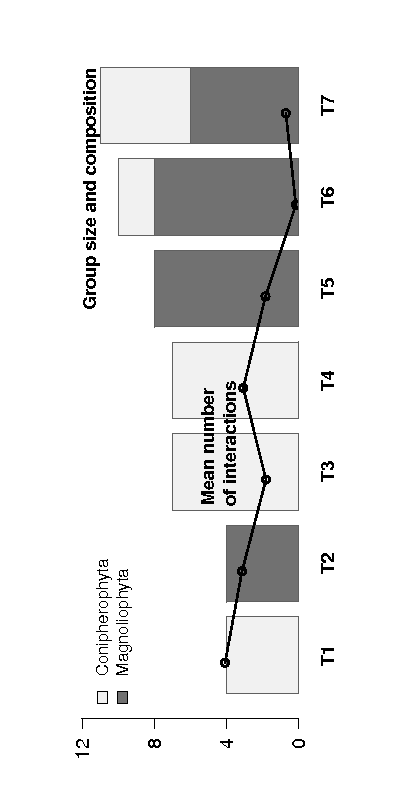
\includegraphics[height=.3\textwidth,width=.25\textwidth,angle=270,origin=c,trim=0 20 0 0]{\fignet/MRV10_AoAS_Q7_group}
 
    &

    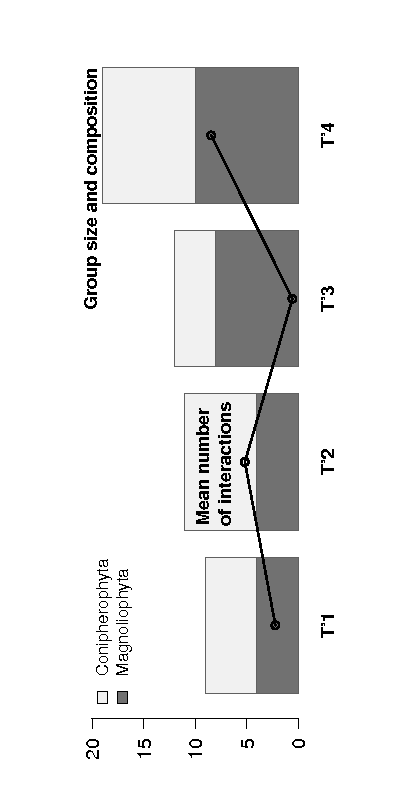
\includegraphics[height=.3\textwidth,width=.25\textwidth,angle=270,origin=c,trim=0 20 0 0]{\fignet/MRV10_AoAS_Q4_group}  
  \end{tabular}

}

%====================================================================
\frame{\frametitle{Sequential importance sampling scheme}

  Consider $\emphase{U = (\theta, Z)}$
  
  \bigskip
  \paragraph{Distribution path:}
    set $0 = \rho_0 < \rho_1 < \dots < \rho_{H-1} < \rho_H = 1$,
  \begin{align*}
     p_h(U) & \propto p_{\text{start}}(U)^{\emphase{{1-\rho_h}}} \; \times \; p_{\text{target}}(U)^{\emphase{{\rho_h}}} \\
     \\
     & \propto p_{\text{start}}(U) \; \times \; r(U)^{\emphase{{\rho_h}}}, 
     & r(U) & = \frac{p(U) p(Y \mid U)}{p_{\text{start}}(U)}
  \end{align*}
  
  \bigskip \bigskip \pause
  \paragraph{Sequential sampling.} At each step $h$, provides
  $$
  \Ecal_h = \{(U_h^m, w_h^m)\}_m = \text{ weighted sample of } p_h
  $$

  \bigskip \pause
  \paragraph{Tune $\rho_{h+1}$} 
  to keep the efficient sample size sufficiently high at each step. \\
  ~ \\
  \ra Doable because $r(U)$ does not depend on $\rho$.

}

%====================================================================
\frame{\frametitle{Sequential sampling: in pictures}  

  \begin{tabular}{cc}
    \hspace{-.04\textwidth}
   \begin{tabular}{p{.5\textwidth}}
      \begin{itemize}
        \onslide+<1->{\item $\textcolor{red}{p_{\text{start}}} = $ proposal, $\textcolor{blue}{p_{\text{target}}} = $ target \\ ~ \\} 
        \onslide+<2->{\item Intermediate distributions
        $p_{\text{start}} = p_0$, $p_1$, $...$, $p_H = p_{\text{target}}$ \\ ~ \\}
        \onslide+<3->{\item Iteratively: \\
        use $p_h$ to get a sample from $p_{h+1}$}
      \end{itemize}
    \end{tabular}
    & 
    \hspace{-.02\textwidth}
    \begin{tabular}{p{.5\textwidth}}
      \begin{overprint}
        \onslide<1> 
        \includegraphics[width=.4\textwidth]{\figbayes/FigVBEM-IS-PropTarget.pdf}
        \onslide<2> 
        \includegraphics[width=.4\textwidth]{\figbayes/FigVBEM-IS-Tempering.pdf}
        \onslide<3> 
        \includegraphics[width=.4\textwidth]{\figbayes/FigVBEM-IS-Tempering-step1.pdf}
        \onslide<4> 
        \includegraphics[width=.4\textwidth]{\figbayes/FigVBEM-IS-Tempering-step2.pdf}
        \onslide<5> 
        \includegraphics[width=.4\textwidth]{\figbayes/FigVBEM-IS-Tempering-step3.pdf}
        \onslide<6-> 
        \includegraphics[width=.4\textwidth]{\figbayes/FigVBEM-IS-Tempering-step4.pdf}
      \end{overprint}
    \end{tabular}
  \end{tabular}  
  
  \bigskip
  \onslide+<7>{+ resampling/propagation to avoid complete degeneracy \refer{DoR19}}

}

%====================================================================
\backupend 

%====================================================================
%====================================================================
\end{document}
%====================================================================
%====================================================================

  \begin{tabular}{cc}
    \hspace{-.04\textwidth}
    \begin{tabular}{p{.5\textwidth}}
    \end{tabular}
    &
    \begin{tabular}{p{.45\textwidth}}
    \end{tabular}
  \end{tabular}

